% !TEX root = ../../sethomas_thesis_main.tex

\documentclass[border=1mm,
               class=article
               preview]{standalone}
\usepackage{tikz}
\begin{document}
\begin{tikzpicture}
  % \node[anchor=south west,inner sep=0] (graph) at (0,0) {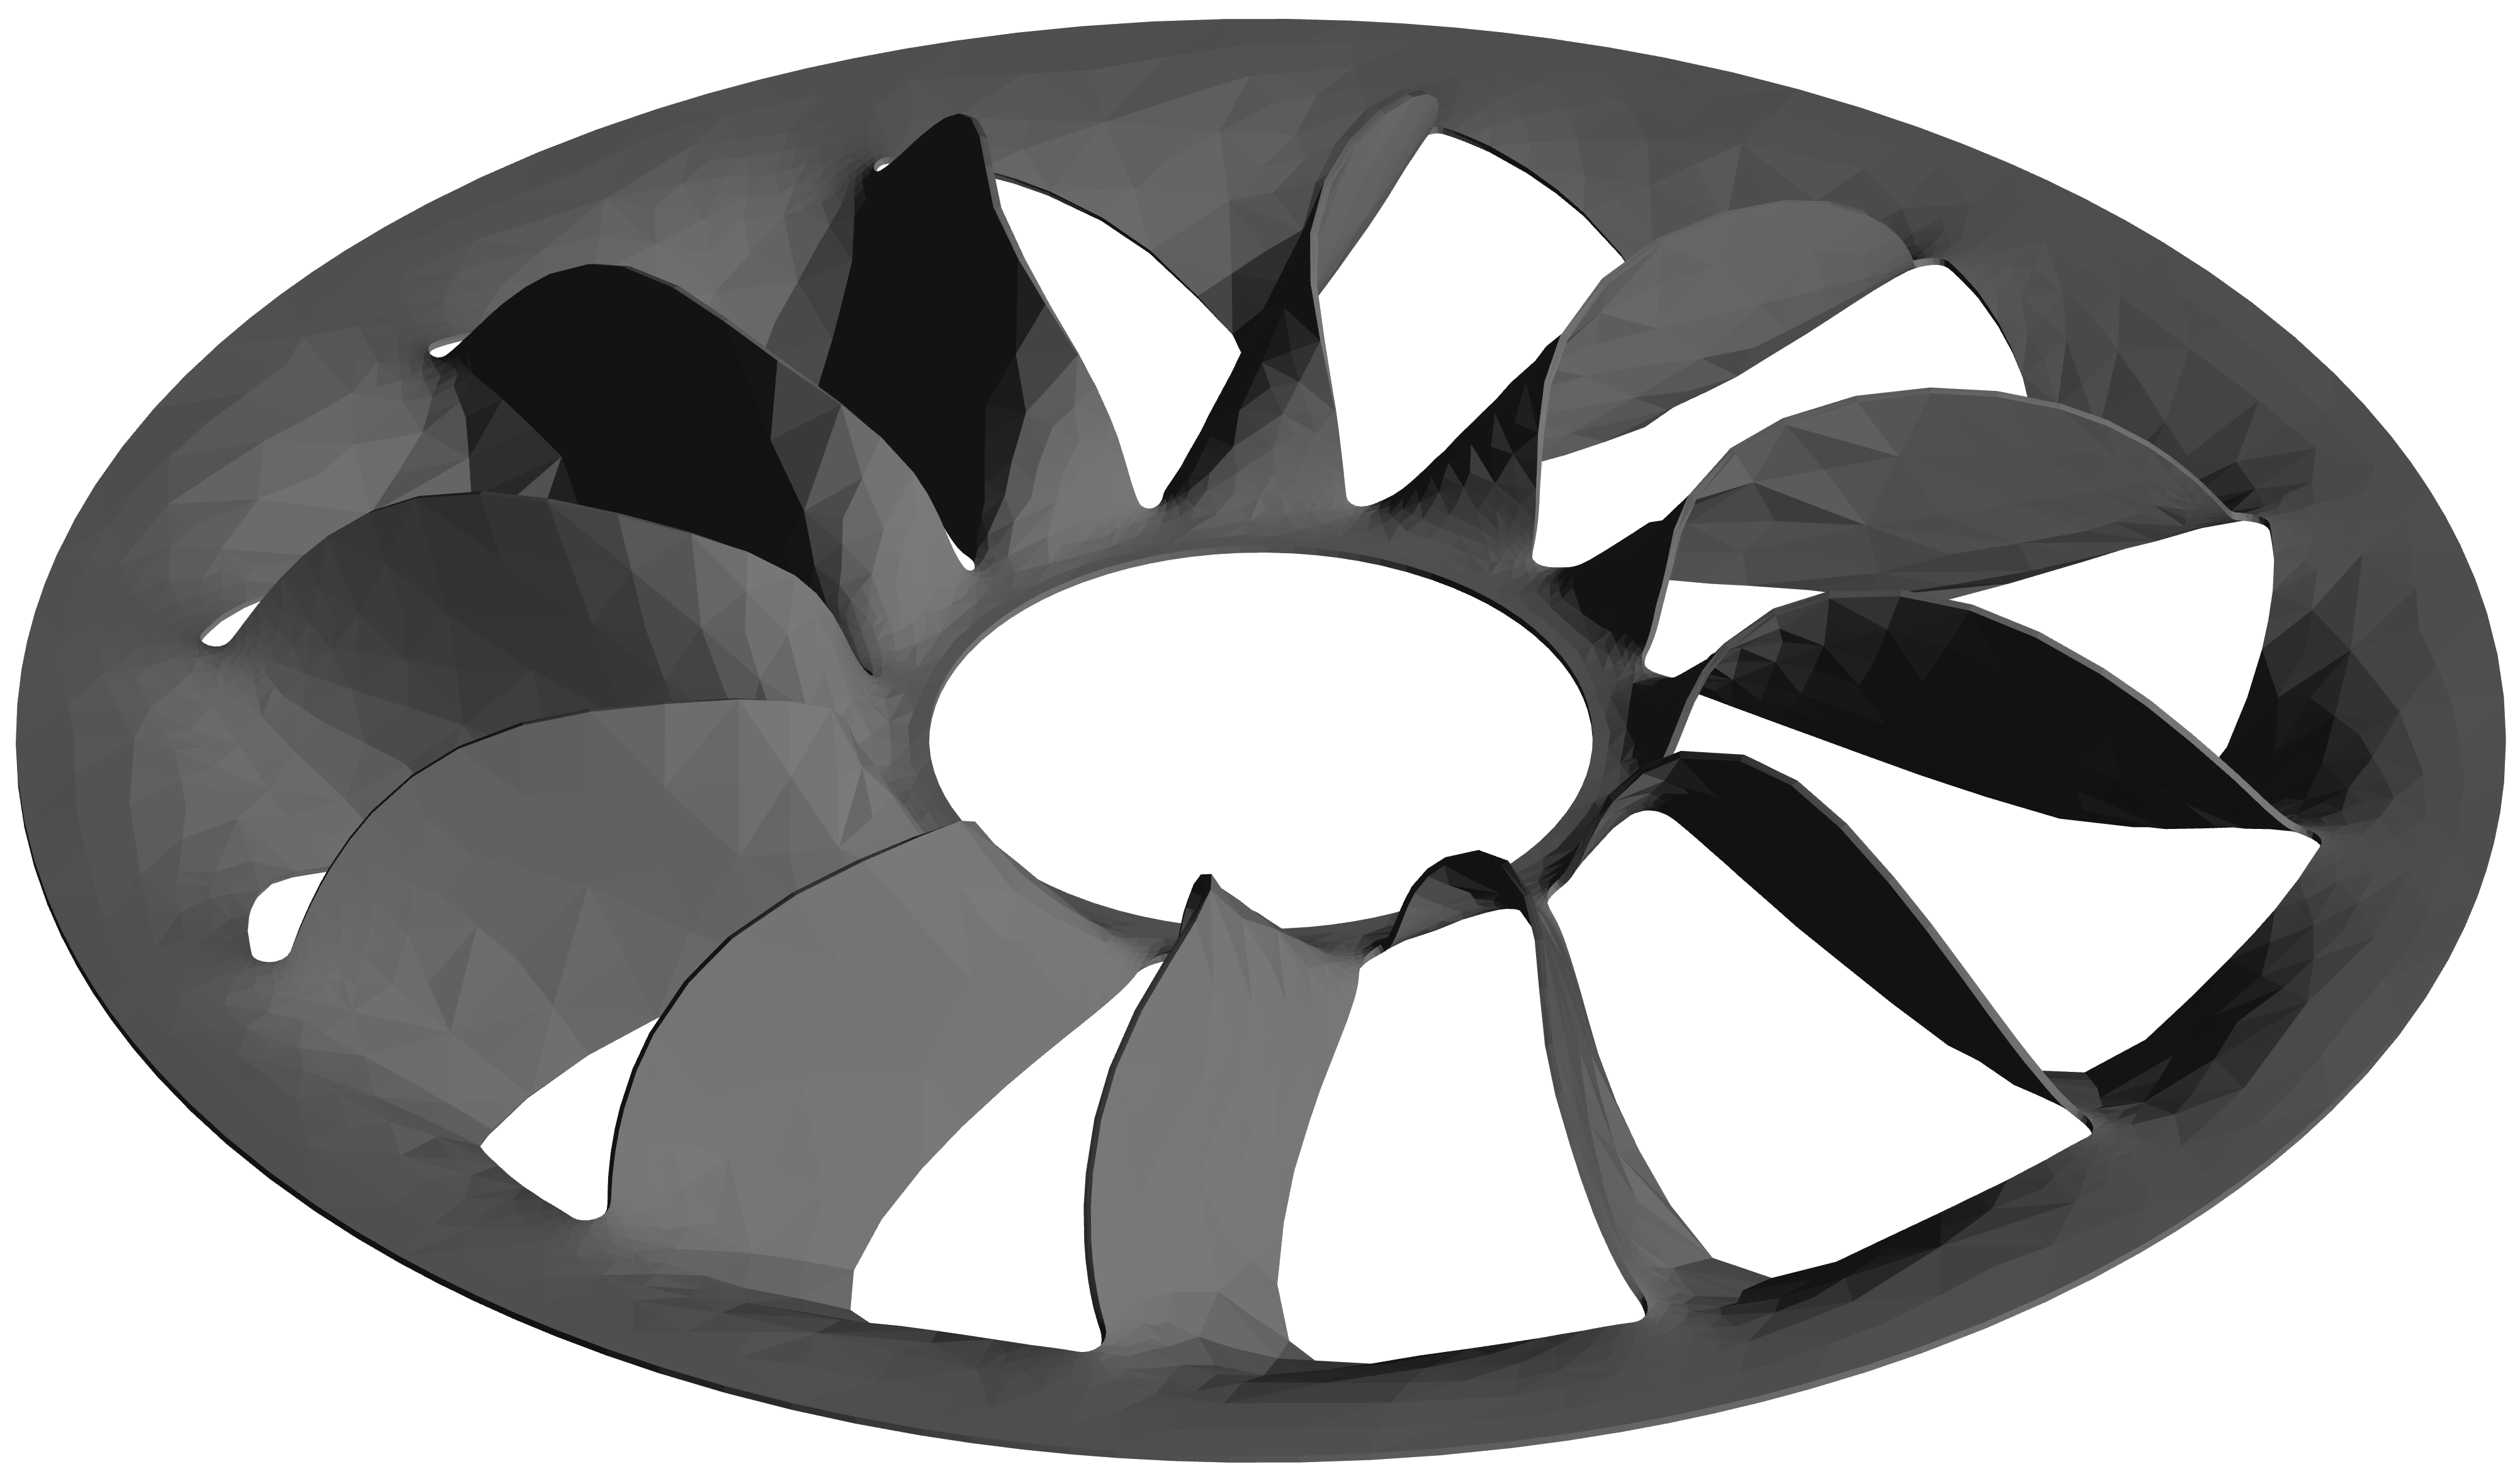
\includegraphics[trim={0 0 0 0},clip]{images/chap5/lotus-kirigami-deformed-contrast.png}};
  \node[anchor=south west,inner sep=0] (graph) at (0,0) {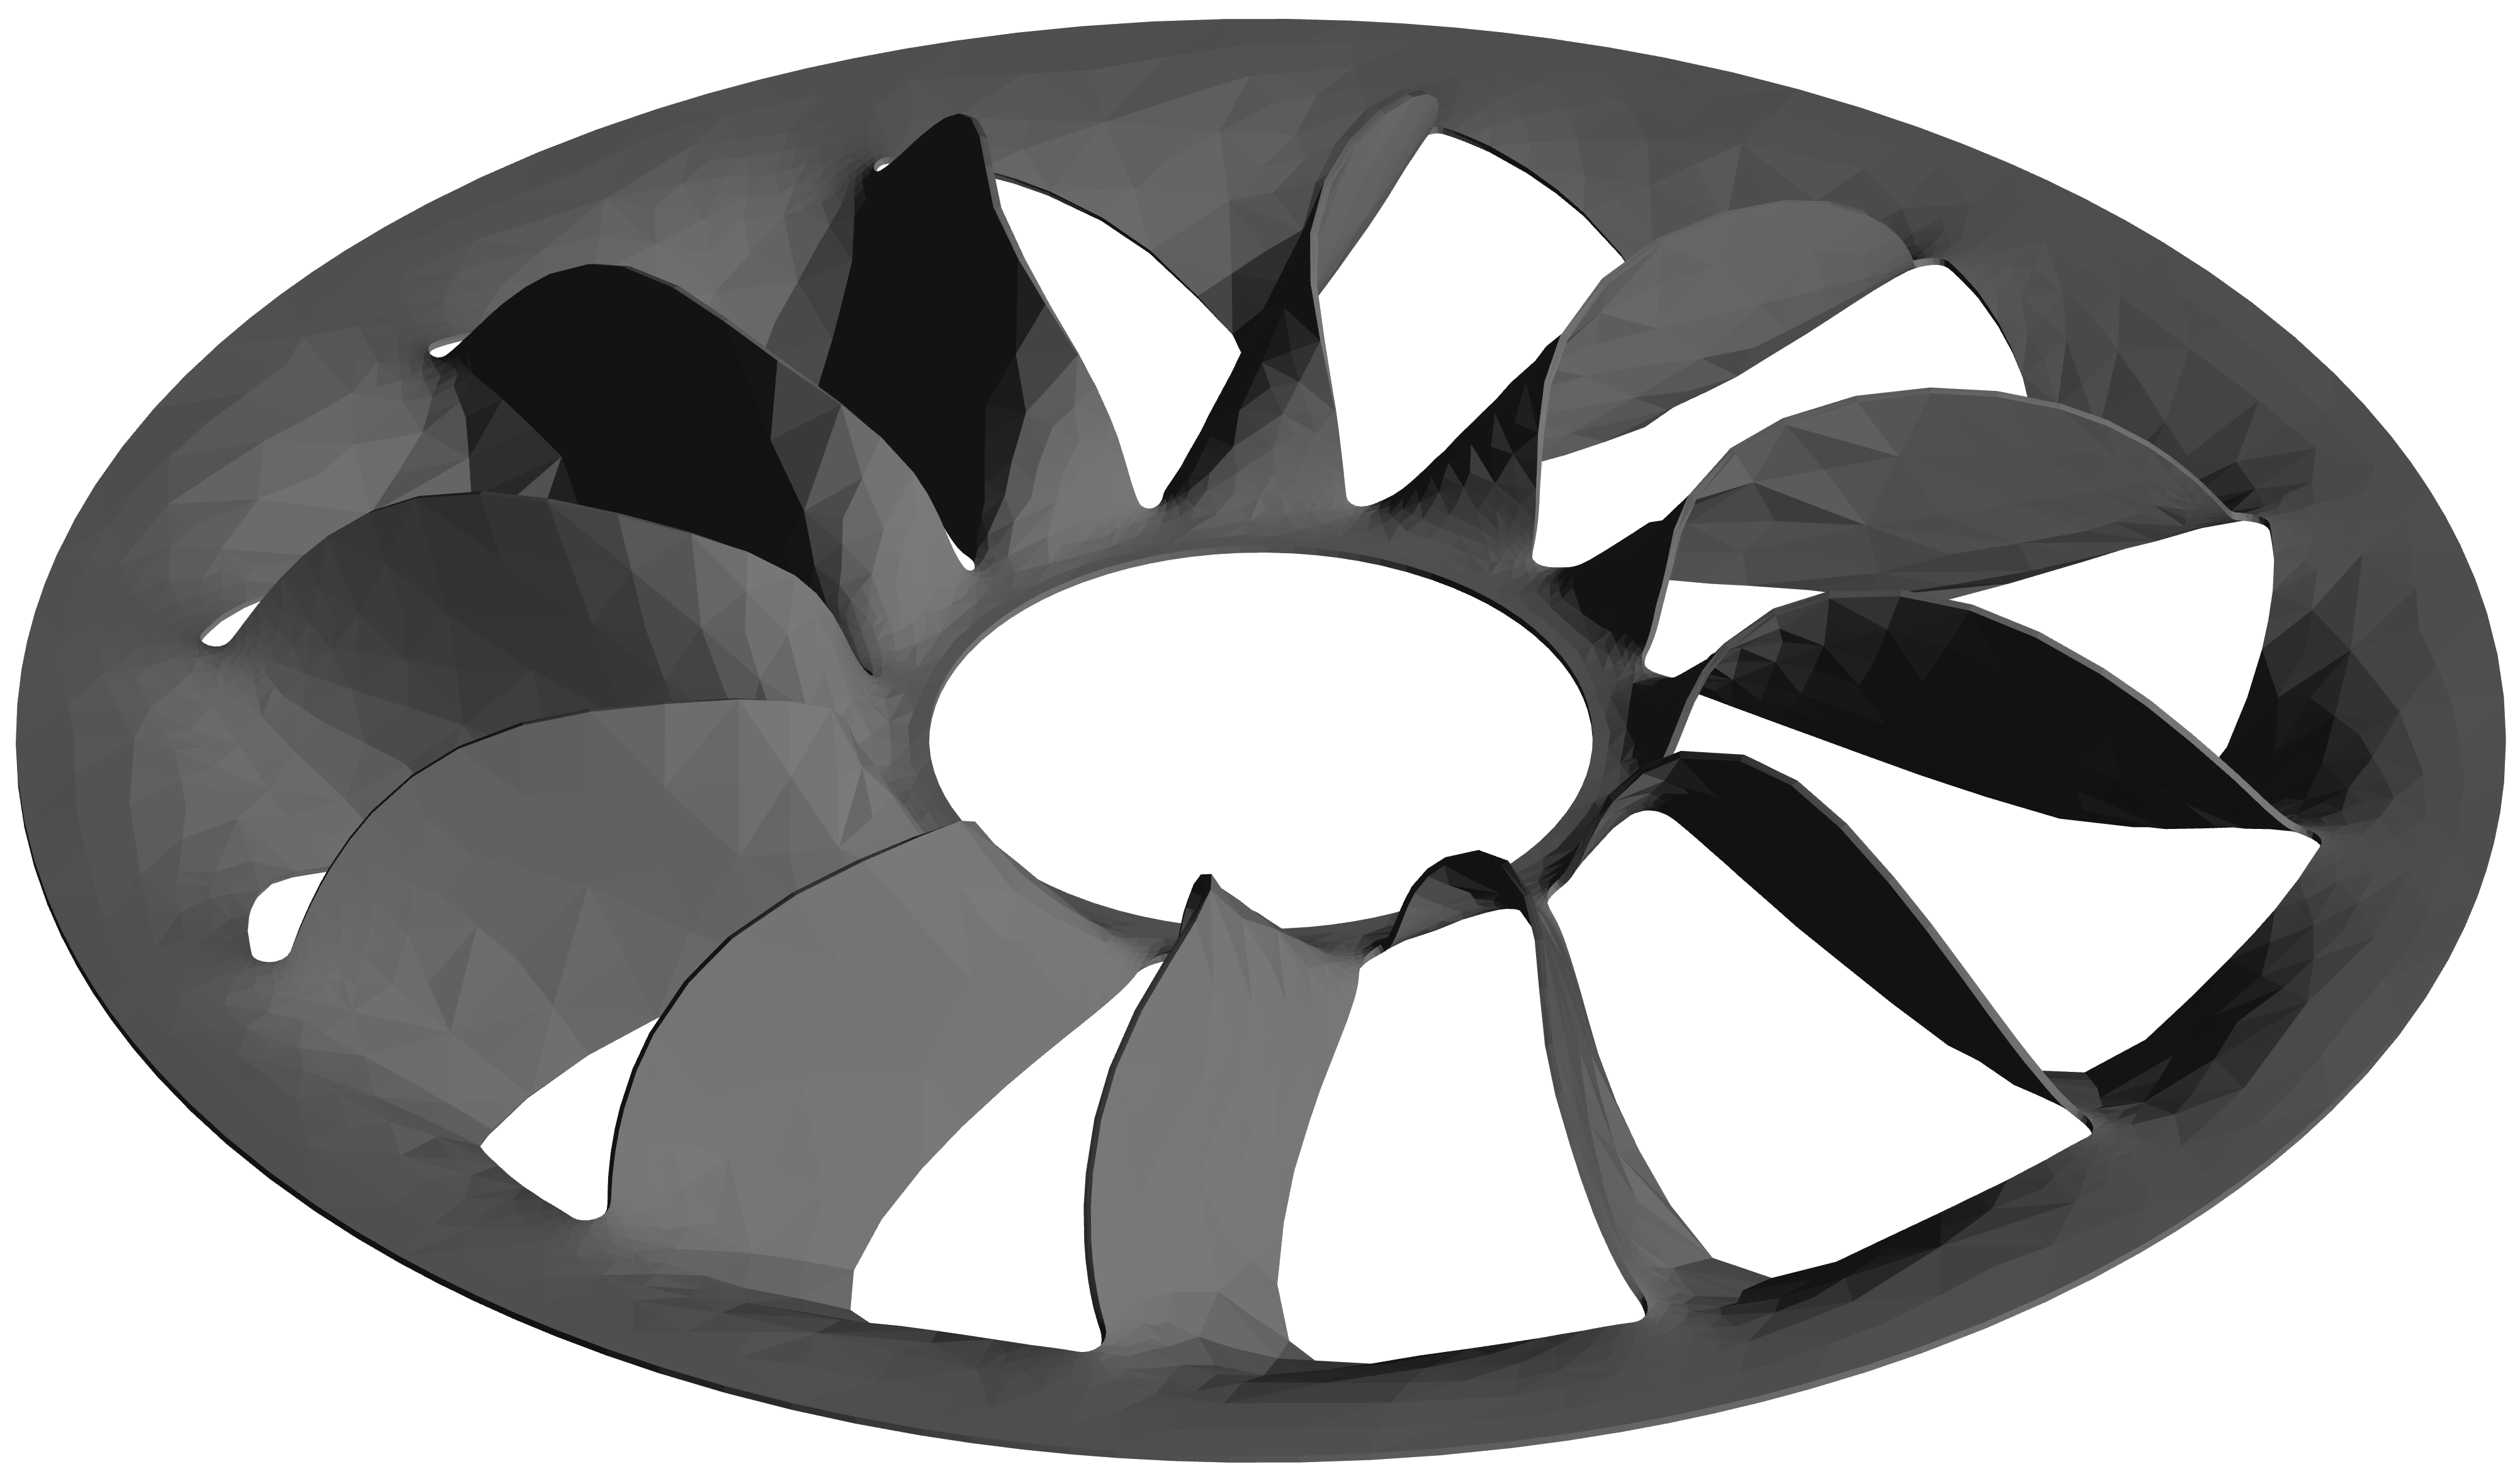
\includegraphics[trim={0 0 0 0},clip, width=0.66\textwidth]{images/chap5/lotus-kirigami-deformed-contrast.png}};

  % \node[anchor=south west,inner sep=0] (graph) at (0,0) {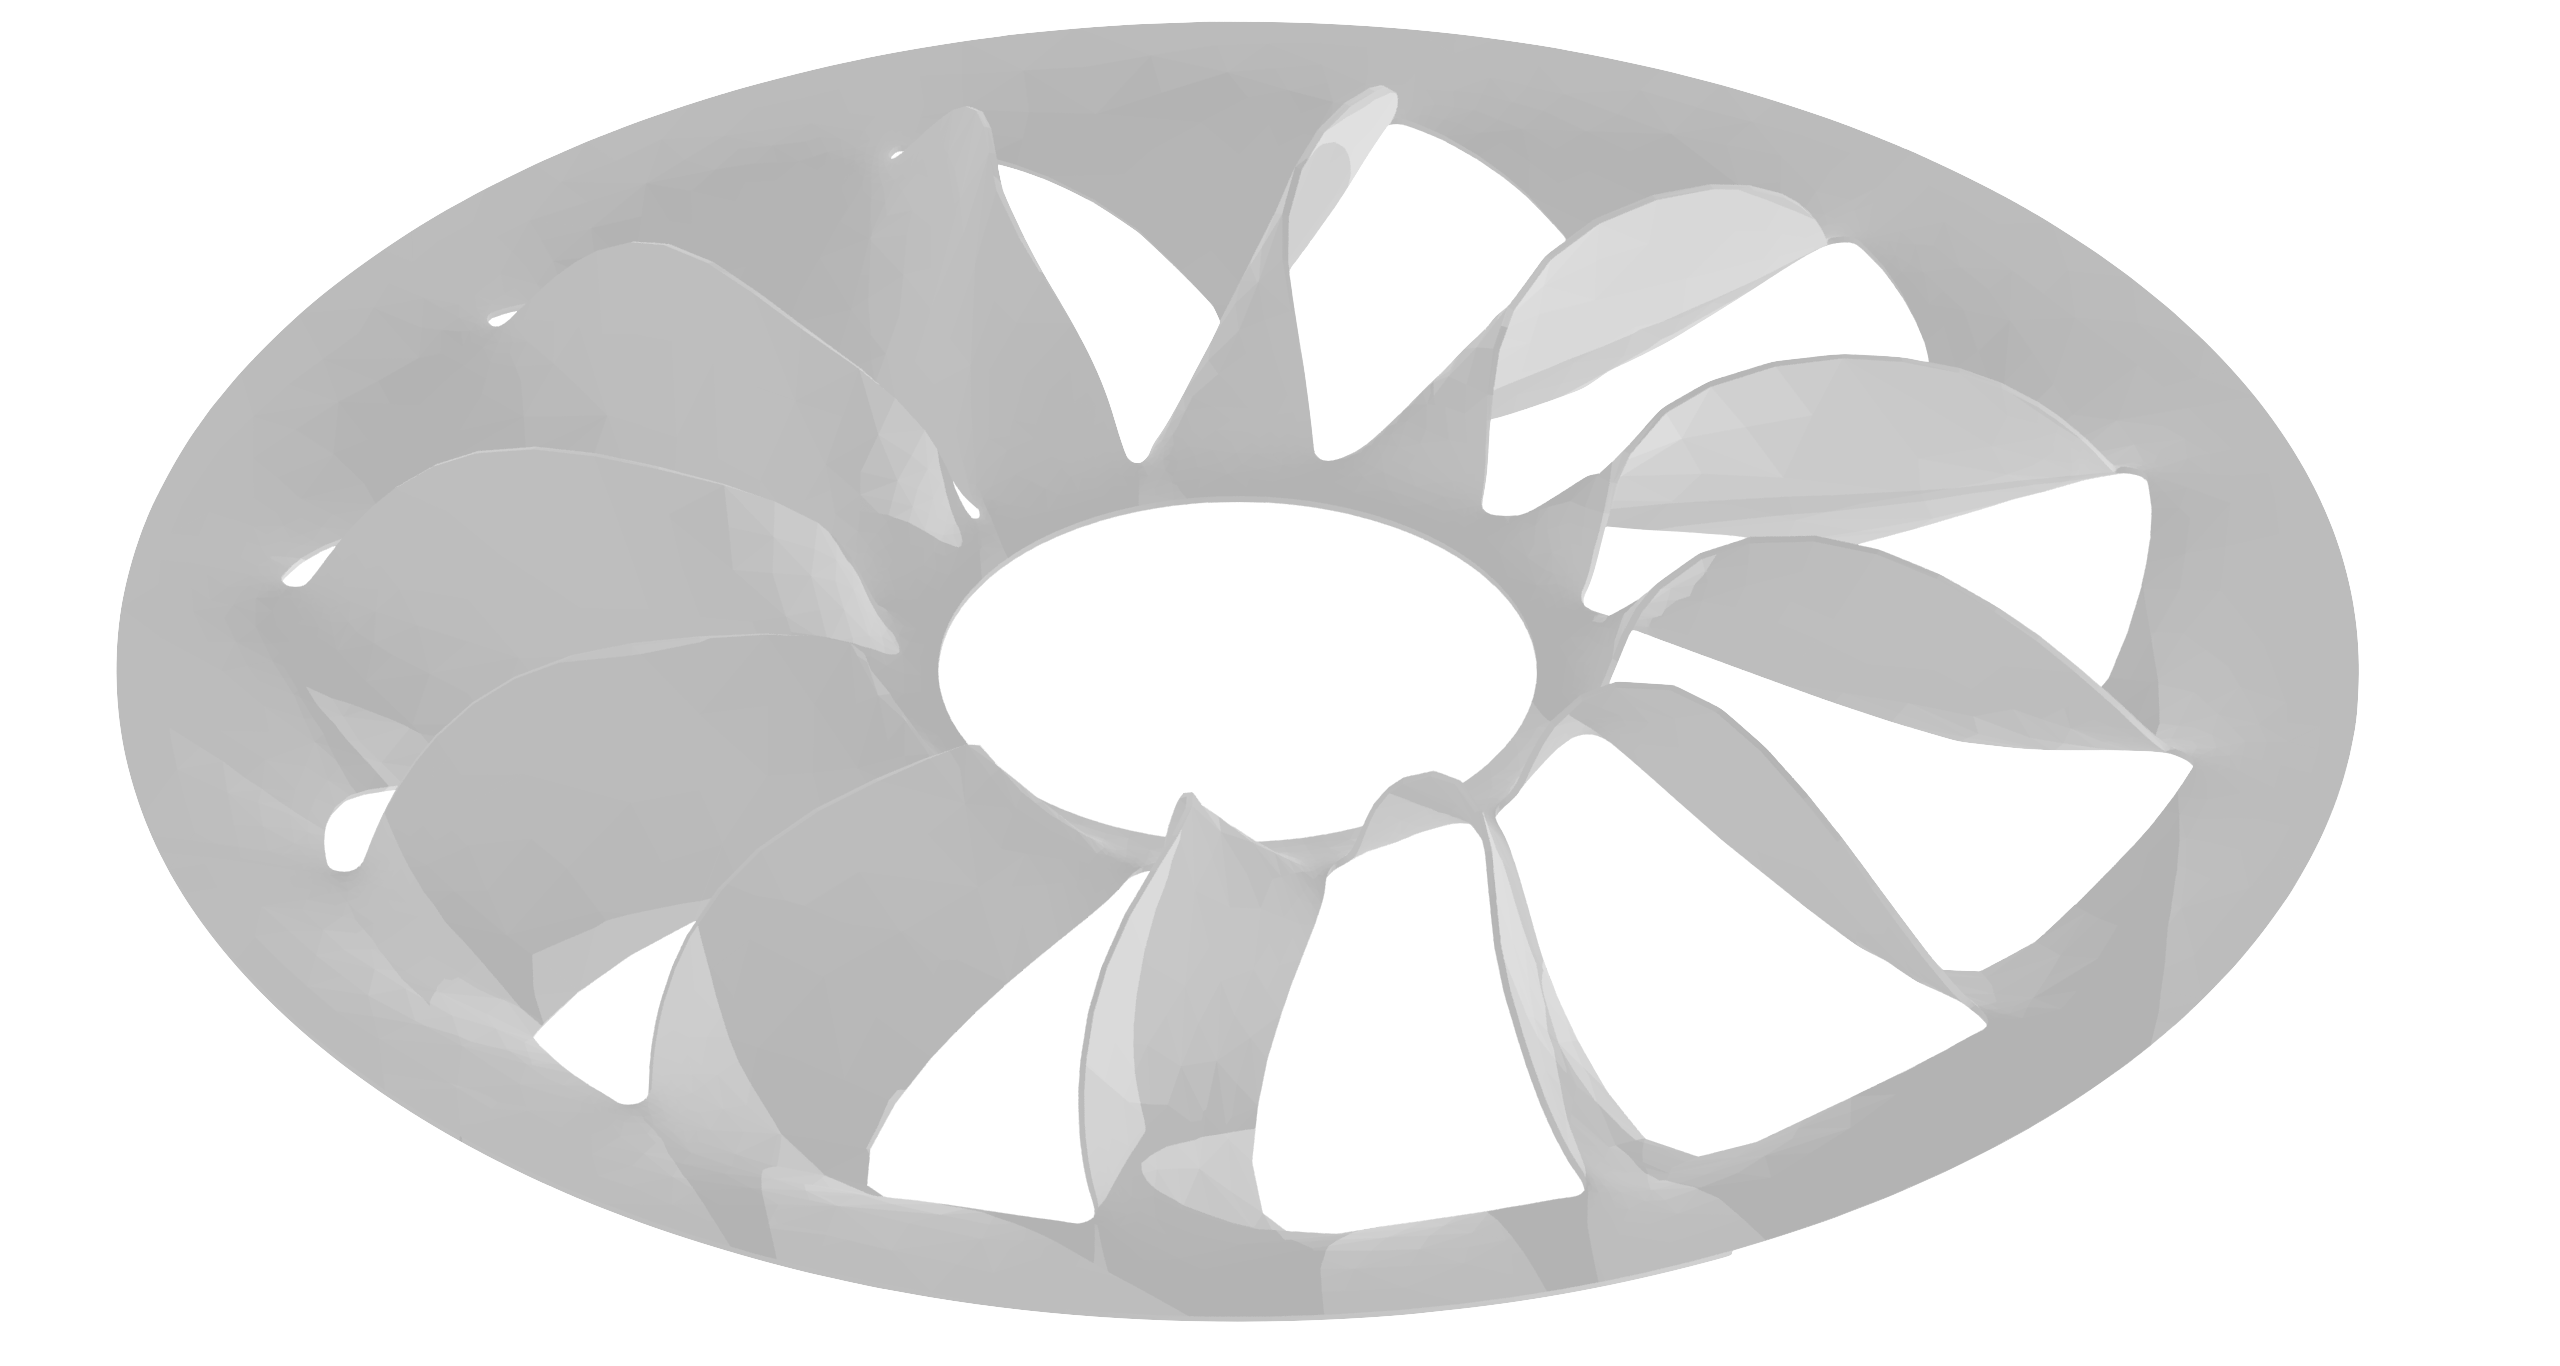
\includegraphics[trim={0 0 0 0},clip, width=0.75\textwidth]{images/chap5/lotus-kirigami-deformed-transp.png}};
  % Insert a relative reference based on image dimensions
  \begin{scope}[x={(graph.south east)},y={(graph.north west)}]
    \draw[-latex,>=stealth',very thick] (0.41,0.57) arc[radius=0.1, start angle=150, end angle=330];
    \node[anchor=center] at (0.50,0.53) (M) {\large$M(\Delta\theta)$};
    % \draw[-latex,>=stealth',very thick] (0.4,0.57) arc[radius=0.09, start angle=150, end angle=330];
    % \node[anchor=center] at (0.48,0.535) (M) {$M(\Delta\theta)$};
  \end{scope}
\end{tikzpicture}
\end{document}
